\section{Лекция 16.02.2018}

\bigskip
\textbf{Лемма.} Пусть $e' = (e'_1, \dots, e'_n)$ -- базис $V$ вида $(*)$. Пусть $\delta'_k = \delta_k(Q, e')$, $k = 1, \dots, n$. Тогда $\delta_k = \delta'_k \ \forall k$.

\bigskip
\textbf{\textit{Доказательство.}} $\rhd \ \forall \ k =1, \dots, n \ <e'_1, \dots, e'_k> = <e_1, \dots, e_k>$. Имеем $B'_k = C_k^T B_k C_k \Rightarrow \delta'_k = det B'_k = det(C_k^T) det B_k det C_k = det B_k = \delta_k \ \lhd$.

\bigskip
\textbf{Теорема 2 (метод Якоби приведения квадратичной формы к каноническому виду).} Предположим, что $\delta_k \neq 0 \ \forall \ k =1, \dots, n$. Тогда $\exists !$ базис $e'$ в $V$, такой что

1) $e'$ имеет вид $(*)$

2) в базисе $e'$ квадратичная форма $Q$ имеет канонический вид $Q(x) = \delta_1 {x'_1}^2 + \frac{\delta_2}{\delta_1} {x'_2}^2 + \dots + \frac{\delta_n}{\delta_{n-1}} {x'_n}^2$ (т.е. $B(Q, e') = diag(\delta_1, \frac{\delta_2}{\delta_1}, \dots, \frac{\delta_n}{\delta_{n-1}}))$.

\bigskip
\textbf{\textit{Доказательство.}} $\rhd$ Индукция по $n$: $n = 1$ -- верно

Пусть доказано для $<n$, докажем для $n$. Пусть векторы $e'_1, \dots, e'_{n-1}$ уже построены (В базисе ($e'_1, \dots, e'_{n-1}, e'_n))$

\begin{equation*} \begin{pmatrix} \delta_1 & 0 & 0 & \dots & 0 & * \\ 0 & \frac{\beta_2}{\beta_1} & 0 & \dots & 0 & * \\ 0 & 0 & \frac{\beta_3}{\beta_2} & \dots & 0 & * \\ \vdots & \vdots & \vdots & \vdots & \vdots & \vdots \\ 0 & 0 & 0 & \dots & \frac{\beta_n}{\beta_{n-1}} & * \\ * & * & * & \dots & * & * \end{pmatrix}
\end{equation*}

\bigskip
Ищем $e'_n$ в виде $e'_n \in e_n + <e_1, \dots, e_{n-1}> = e_n + <e'_1, \dots, e'_{n-1}>$, т.е. $e'_n = e_n + \lambda_1 e'_1 + \lambda_2 e'_2 + \dots + \lambda_{n-1} e'_{n-1}$

Пусть $\beta$ -- симметричная билинейная форма, соответствующая квадратичной ворме $Q$

$\forall k = 1, \dots, n-1$ имеем 

$\beta(e'_n, e'_k) = \beta(e_n, e'_k) + \lambda_1 \beta(e'_1, e'_k) + \dots + \lambda_{n-1} \beta(e'_{n-1}, e'_k) = \beta(e_n, e'_k) + \lambda_k \beta(e'_k, e'_k) =\beta(e_n, e'_k) + \lambda_k \frac{\beta_k}{\beta_{k-1}} $

\bigskip
Тогда $\beta(e'_n, e'_k) = 0 \Leftrightarrow \lambda_k = -\beta(e_n, e'_k) \cdot \frac{\delta_{k-1}}{\delta_{k}}$. Теперь в базисе $e' = (e'_1, \dots, e'_n)$.

\begin{equation*} B(Q, e') = \begin{pmatrix} \delta_1 & 0 & 0 & \dots & 0 & 0 \\ 0 & \frac{\beta_2}{\beta_1} & 0 & \dots & 0 & 0 \\ 0 & 0 & \frac{\beta_3}{\beta_2} & \dots & 0 & 0 \\ \vdots & \vdots & \vdots & \vdots & \vdots & \vdots \\ 0 & 0 & 0 & \dots & \frac{\beta_{n-1}}{\beta_{n-2}} & 0 \\ 0 & 0 & 0 & \dots & 0 & ? \end{pmatrix}
\end{equation*}

\bigskip
По лемме имеем $\delta_n = \delta'_n \Rightarrow \delta_n = \delta'_n = \delta_1 \frac{\delta_2}{\delta_1} \dots \frac{\delta_{n-1}}{\delta_{n-2}} \cdot ? = \delta_{n-1} \cdot ? \Rightarrow ? = \frac{\delta_n}{\delta_{n-1}}$.

Единственность следует из явных формул для $e'_k, k = 1, \dots, n \ \lhd$

\bigskip
\textbf{Замечание.} При $\beta_k \neq 0 \ \forall \ k = 1, \dots, n$ метод Лагранжа и метод Якоби дают один и тот же результат. 

\bigskip
\textbf{Определение.} Говорят, что \textit{квадратичная форма $Q$ имеет в базисе $e$ нормальный вид}, если $Q$ имеет в $e$ канонический вид $Q(x) = b_1 x_1^2 + \dots + b_n x_n^2$, где $b_i \in \{-1, 0, 1\}$.

\bigskip
\textbf{Следствие из теоремы 1 (метод Лагранжа).} Если $F = \RR$, то $\forall$ квадратичной формы $Q \ \exists$ базис, в котором $Q$ имеет нормальный вид.

\bigskip
\textbf{\textit{Доказательство.}} Теорема 1 $\Rightarrow \ \exists$ базис $e$, в котором $Q(x) = b_1 x_1^2 + \dots + b_n x_n^2$. Сделаем замену

$ x_i = \begin{cases}
		\frac{x_i}{\sqrt[]{|b_i|}}, \ если \ b_i \neq 0 \\
		x'_i, \ если \ b_i = 0
	\end{cases}$

Тогда в новых координатах $Q(x) = \varepsilon_1 {x'_1}^2 + \dots + \varepsilon_n {x'_n}^2$, где $\varepsilon_i = sgn(b_i) = \begin{cases}
		1, b_i > 0 \\
		0, b_i = 0 \\
        -1, b_i < 0 
	\end{cases} \ \lhd$
    

\bigskip
\textbf{Замечание.} Аналогичные рассуждения показывают, что для $F = \CC \ \forall$ квадратичной формы $Q \exists$ базис, в котором $Q$ имеет вид $x_1^2 + \dots + x_k^2, k = rkQ$.

\bigskip
Пусть квадратичная форма $Q$ имеет в базисе $e$ нормальный вид $Q(x) = x_1^2 + \dots + x_s^2 - x_{s+1}^2 - \dots - x_{s+t}^2$, $s$ -- число "+" в нормальном виде, $t$ -- число минусов в нормальном виде

\bigskip
\textbf{Теорема (закон инерции).} Числа $i_+ = s$ и $i_- = t$ не зависят от базиса, в котором $Q$ имеет нормальный вид.

\bigskip
\textbf{\textit{Доказательство.}} $\rhd$ Пусть базисы $e$ и $e'$ таковы, что 

в $e$ $Q(x) = x_1^2 + \dots + x_s^2 - x_{s+1}^2 - \dots - x_{s+t}^2$

в $e'$ $Q(x) = {x'_1}^2 + \dots + {x'_{s'}}^2 - {x'_{s'+1}}^2 - \dots - {x'_{s'+ t'}}^2$

Имеем $s + t = rkQ = s' + t' \Rightarrow$ достаточно доказать, что $s = s'$. Предположим, $s \neq s'$. Без ограничения общности можно определить, что $s > s'$.

Рассмотрим подпространства $L_1 = <e_1, \dots, e_s>$ и $L_2 = <e'_{s'+1}, \dots, e'_n>$, $dimL_1 = s, dimL_2 = n-s'$

$L_1 + L_2 \subseteq V \Rightarrow dim (L_1 + L_2) \leq n$.

Тогда $dim(L_1 \cap L_2) = dimL_1 + dimL_2 - dim(L_1 + L_2) \geq s + n - s' = s - s'> 0 \Rightarrow \exists v \in L_1 \cap L_2 \setminus \{0\} $

Т.к. $v \in L_1$, то $Q(v) > 0$

т.к. $v \in L_2$, то $Q(v) \leq 0$

противоречие $\lhd$.

\bigskip
\textbf{Определение.} $i_+$ называется \textit{положительным индексом инерции квадратичной формы} $Q$, $i_-$ называется \textit{отрицательным индексом инерции квадратичной формы} $Q$.

\bigskip
\textbf{Следствие метода Якоби.} Пусть $e$ -- базис, $\delta_k \neq 0 \ \forall \ k \Rightarrow$ число $i_-$ равно количество перемен знака в последовательности $1, \delta_1, \delta_2, \dots, \delta_n$.

\bigskip
\textbf{\textit{Доказательство.}} $\rhd$ Метод Якоби $\Rightarrow$ канонический вид $Q(x) = \frac{\delta_1}{\delta_0} x_1^2 + \frac{\delta_2}{\delta_1} x_2^2 + \dots + \frac{\delta_n}{\delta_{n-1}} x_n^2$ ($\delta_0 = 1$)

$\frac{\delta_k}{\delta_{k-1}} < 0 \Leftrightarrow \delta_k$ и $\delta_{k-1}$ имеют разные знаки $\lhd$.

\bigskip
\textbf{Определение.} Квадратичная форма называется 

\bigskip
\begin{center}
		\begin{tabular}{c|c|c}
    	Термин & Обозначение & Условие   \\
        \hline
        Положительно определенной & $Q > 0$ & $Q(x) > 0 \ \forall \ x \neq 0$ \\
        Отрицательно определенной & $Q < 0$ & $Q(x) < 0 \ \forall \ x \neq 0$ \\
        Неотрицательно определенной & $Q \geq 0$ & $Q(x) \geq 0 \ \forall \ x$ \\
        Неположительно определенной & $Q \leq 0$ & $Q(x) \leq 0 \ \forall \ x$ \\
        Неопределенной & - & $\exists x: Q(x) > 0, \exists y: Q(y) < 0$ 
        
		\end{tabular}
\end{center}
\begin{center}
		\begin{tabular}{c|c}
    	Нормальный вид & Индексы инерции   \\
        \hline
        $x_1^2 + \dots + x_n^2$ & $i_+ = n, i_- = 0$ \\
        $-x_1^2 - \dots - x_n^2$ & $i_+ = 0, i_- = n$ \\
        $x_1^2 + \dots + x_n^2, k \leq n$ & $i_+ = k, i_- = 0$ \\
        $-x_1^2 - \dots - x_n^2, k \leq n$ & $i_+ = 0, i_- = k$ \\
        $x_1^2 + \dots + x_s^2 - x_{s+1}^2 - \dots - x_{s+t}^2, \ s, t \geq 1$ & $i_+ = s \geq 1, i_- = t \geq 1$ 
		\end{tabular}
\end{center}

\bigskip
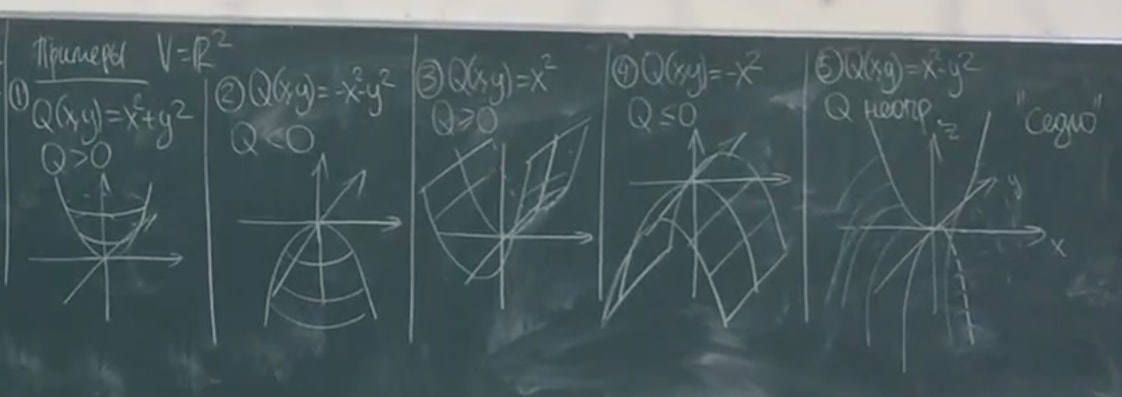
\includegraphics[width=18cm,height=14cm,keepaspectratio]{examples.jpg}

\bigskip
\textbf{\textit{Применение.}}

$f : R^n \rightarrow R$, $x_0 \in R^n$

$x = x_0 + y, \ y \in R^n$ -- "малое приращение"

Предположим, что в окрестности точки $x_0 \ f$ представима в виде $f(x) = f(x_0) + a_1 y_1 + \dots + a_n y_n + b_1 y_1^2 + \dots + b_n y_n^2 + \sum\limits_{1 \leq i < j \leq n} 2 b_{ij} y_i y_j + O(|y|^2)$, где $a_1 y_1 + \dots + a_n y_n = l(y)$ -- линейная форма, а $b_1 y_1^2 + \dots + b_n y_n^2 + \sum\limits_{1 \leq i < j \leq n} 2 b_{ij} y_i y_j = Q(y)$ -- квадратичная форма.

\bigskip
\textbf{Теорема.} 1) Если $f$ имеет в точке $x_0$ экстремум, то $l(y) = 0$

2) Пусть $l(y) = 0$. Тогда если $Q(y) > 0$, то $f$ имеет локальный минимум в точке $x_0$

если $Q(y) < 0$, то $f$ имеет локальный максимум в точке $x_0$

если $Q(y)$ неопределенная, то экстремума нет

